\documentclass[12pt]{article}
\usepackage{amsmath,amsthm,amssymb,amsfonts}
\usepackage{setspace,enumitem}
\usepackage{graphicx}
\usepackage{setspace}
\usepackage{hyperref}
\usepackage{natbib}
\usepackage{afterpage}
\usepackage{xcolor}
\usepackage{etoolbox}
\usepackage{booktabs}
\usepackage{pdfpages}
\usepackage{multicol}
\usepackage{geometry}
\usepackage{accents}
\usepackage{bbm}
\usepackage{placeins}
\usepackage[affil-it]{authblk} 
\hypersetup{
	colorlinks,
	linkcolor={blue!90!black},
	citecolor={red!90!black},
	urlcolor={blue!90!black}
}

\newtheorem{theorem}{Theorem}
\newtheorem{assumption}{Assumption}
\newtheorem{definition}{Definition}
\newtheorem{lemma}{Lemma}
\geometry{margin = 1in}

\newcommand{\R}{\mathbb{R}}
\newcommand{\ubar}[1]{\underaccent{\bar}{#1}}
\newcommand{\Int}{\text{Int}}
\newcommand{\xbf}{\mathbf{x}}
\newcommand{\Abf}{\mathbf{A}}
\newcommand{\Bbf}{\mathbf{B}}
\newcommand{\Gbf}{\mathbf{G}}
\newcommand{\bbf}{\mathbf{b}}
\newcommand{\one}{\mathbbm{1}}

\newtoggle{extended}
\settoggle{extended}{false}

\title{Optimal Capital Requirements with Private Information}
\author{Alex von Hafften}

\begin{document}

\maketitle

\doublespacing

Determining the optimal level of bank capital requirement is an important and well-researched area.  Deposit insurance create moral hazard through limited liability. This moral hazard encourages banks to take on excessive risk and become larger than socially optimal.  Capital requirements are the primary regulatory tool to address moral hazard and limit banks' capacity to use deposit and debt financing.  However, many recent quantitative general equilibrium models (e.g., Pandolfo ~\cite{pandolfo_2021}, Corbae and Levine ~\cite{corbae_levine_2022}, Corbae and D'Eramso ~\cite{corbae_derasmo_2021}) omit the possibility that banks have more information about the riskiness of their loan than regulators.  In this paper, I augment Pandolfo ~\cite{pandolfo_2021} so that banks receive an informative private signal about the riskiness of their loan.  I plan to estimate the strength of the signal using simulated method of moments to match the cross-sectional correlation between lagged loan growth and realized loan returns.

\section{Literature Review}

My paper relates to a number of literatures on banking.  First, it relates to literature on deposit insurance.  Seminal papers at Diamond and Dybvig ~\cite{diamond_dybvig_1983} shows how a bank's illiquid assets and liquid liabilities may rise in self-fulfilling bank runs. They show that deposit insurance can prevent such runs.  Kareken and Wallace ~\cite{kareken_wallace_1978} argue that deposit insurance lead banks to take on excessive risk by creating moral hazard through limited liability.  

\pagebreak

Second, my paper relates the literature on quantitative general equilibrium models of banking.  A number of recent studies including Van der Heuvel ~\cite{vandenheuvel_2008}, De Nicolo et al ~\cite{denicolo_2014}, Faira e Castro ~\cite{fariaecastro_2020}, Begenau and Landvoigt ~\cite{begenau_landvoigt_2021}, Bianchi and Bigio ~\cite{bianchi_bigio_2021}, Corbae and D'Eramso ~\cite{corbae_derasmo_2021}, Pandolfo ~\cite{pandolfo_2021}, and Corbae and Levine ~\cite{corbae_levine_2022} use quantitative dynamic general equilibrium models to evaluate capital requirements.  Van der Heuvel ~\cite{vandenheuvel_2008} pioneered this general equilibrium approach.  De Nicolo et al ~\cite{denicolo_2014} and Pandolfo ~\cite{pandolfo_2021} jointly study capital and liquidity requirements. Faira e Castro ~\cite{fariaecastro_2020} incorporates the effects of time-varying capital requirements (i.e., the countercyclical capital buffer).  Begenau and Landvoigt ~\cite{begenau_landvoigt_2021} include the shadow banking system, so tighter bank regulations can shift lending to the shadow banking system. Bianchi and Bigio ~\cite{bianchi_bigio_2021} evaluates the effects of monetary policy within this framework. Corbae and D'Eramso ~\cite{corbae_derasmo_2021} and Corbae and Levine ~\cite{corbae_levine_2022} incorporate an imperfectly competitive banking system and evaluates capital requirements that vary by bank size (i.e. the global systemically important bank capital surcharge).

\bigskip

Third, my paper relates to literature on bank opacity.  Using a theoretical model, Dang et al. ~\cite{dang_2017} argue that banks with private information about the asset-side of their balance can fund NPV positive projects that could not be funded by a more opacity institution like through a capital market.  They argue that it may be optimal for banks to hide information about their asset risks because it allows for efficient coordination that would not exist without that opacity. Their model does not include moral hazard.

\bigskip

My paper is most similar to Pandolfo ~\cite{pandolfo_2021}. I start by simplifying the banks problem from Pandolfo ~\cite{pandolfo_2021} and to limit the focus to capital requirements (i.e., Pandolfo ~\cite{pandolfo_2021} also considers liquidity requirements). Then I add an informative private signal about the loan return before the bank chooses the size of its loan portfolio. If the correlation between the signal and the return is zero, the resulting model is a simplified version of Pandolfo ~\cite{pandolfo_2021}.  If the correlation between the signal and the return is perfect, then the bank perfectly knows its return before it makes its investment.

\pagebreak

Finally, my paper is related to the literature on dynamic private information, in particular Atkeson and Lucas ~\cite{atkeson_lucas_1992}.  The setup that I explore here is isomorphic to a model similar to the dynamic private information model of Mirrleesian taxation.

\section{Model}

\subsection{Simplified Version of Pandolfo ~\cite{pandolfo_2021}}

Pandolfo ~\cite{pandolfo_2021} studies a dynamic general equilibrium banking model. Each period, the bank wakes up with net worth $n$.  It chooses the amount of dividends to pay households $div$, deposits to borrow $d$, and loans to make $L$.  The net worth $n$ and deposit $d$ need to finance its loans $L$, origination costs $\theta \frac{L^2}{2}$ and dividends $div$.  The bank is subject to a capital requirement such that its equity $L - d$ over its loans $L$ must be a larger than some number $\phi$.  I vary $\phi$ to see how welfare changes. The loans are invested in an exogenous production technology with interest rate $i$ that is normally distributed with mean $\mu$ and variance $\sigma^2$.  Net worth evolves as the gross return on the loan portfolio net of the deposit return.  The bank enjoys limited liability, so its continuation value is restricted to be nonnegative. If a bank exits, it is replaced by a bank with the same net worth $n$, which is raised as a lump-sum tax from households. Bank maximizes present discounted value of dividends to shareholders. The banks problem is below:

\begin{align*}
V(n) = \max_{div, d, L} \Big\{ div &+ \beta E [\max\{0, V(n')\}]\Big\} \\
\text{s.t. } 
n + d &= L + \theta \frac{L^2}{2} + div\\
\frac{L - d}{L} & \ge \phi\\
n' &= (1 + i)L - R \cdot d \\
i &\sim N(\mu,\sigma)
\end{align*}

The government resolves defaulted banks. If a bank exits, the government can sell the loans with haircut $1 - \xi$.  Thus, bankruptcy involves a real resource cost on the economy.  The government settles its budget constraint with lump-sum taxes and transfers on households.

\bigskip

There is a unit mass of households that make a consumption-savings decision. They enter the period with net worth $n$ and spend it on consumption $c$, deposits $d$, and buying shares of equity in the bank $e$.  Net worth evolves as the sum of the gross return on their deposits $Rd$, gross return on their holding of the bank $e (p + div)$, lump-sum government taxes/transfers, and endowment $\omega$. 

\begin{align*}
W(n) &= \max_{c, d, e} u(c) + \beta W(n')\\
\text{s.t. } 
c + d + e p &= n\\
n' &= Rd + e (p + div) + T + \omega
\end{align*}

A recursive competitive equilibrium are household and bank value and policy functions such that households optimize, banks optimize, government budget constraint holds, and markets clear.

\subsection{With Informative Private Signals about Loan Return}

I extend the simplified version of Pandolfo ~\cite{pandolfo_2021} to include informative private signals about the shocks to loan returns.  Let loan return shock $\varepsilon$ and signal $m$ be jointly standard normal with correlation $\rho$ that are iid over time.  With this signal, the bank problem becomes:

\begin{align*}
V(n, m) = \max_{div, d, L} \Big\{ div &+ \beta E [\max\{0, V(n', m')\}]\Big\} \\
\text{s.t. } 
n + d &= L + \theta \frac{L^2}{2} + div\\
\frac{L - d}{L} & \ge \phi\\
n' &= (1 + i)L - R \cdot d \\
\begin{pmatrix} i \\ m \end{pmatrix} &\sim N \Bigg( \begin{pmatrix} \mu \\ 0 \end{pmatrix} , \begin{pmatrix} \sigma & \sigma \rho \\ \sigma\rho & 1\end{pmatrix} \Bigg)
\end{align*}

Notice that, based on their signal $m$, the bank updates the parameters which they use to evaluate their expected continuation value:

\begin{align*}
\hat\mu &=  \mu + \sigma \rho m\\
\hat\sigma^2 &=  (1 - \rho^2)\sigma^2
\end{align*}

Thus, we can express the bank problem where the expected return conditional on the signal is the state variable and the interest rate is normally distributed with parameters $\hat\mu$ and $\hat\sigma$.

\begin{align*}
V(n, \hat\mu) = \max_{div, d, L} \Big\{ div &+ \beta E [\max\{0, V(n', m')\}]\Big\} \\
\text{s.t. } 
n + d &= L + \theta \frac{L^2}{2} + div\\
\frac{L - d}{L} & \ge \phi\\
n' &= (1 + i)L - R \cdot d \\
i &\sim N(\hat\mu, \hat\sigma^2)
\end{align*}

With the bank problem in this form, it is clearly that this setup is isomorphic to a dynamic private information problem where there is a continuum of bank types (iid over time) that index the expected return of the loan technology, similar to Atkeson and Lucas ~\cite{atkeson_lucas_1992}.  In line with Atkeson and Lucas ~\cite{atkeson_lucas_1992}, an extension of this setup that I hope to explore is to include banks reporting their type to the regulator and capital requirements being a function of their reported type $\phi(\hat\mu)$.  Such a setup would allow for dynamic incentives (i.e. a report of a low type is punished with more stringent regulation today but rewarded with higher promised utility and a report of high type is reward with looser regulation today but punished with lower promised utility) that is understudied in bank capital requirements.

\bigskip

The intuition for why private informative signals might change the optimal level of capital requirement is that that limited liability has more bit with low signals.  For example, see the figures below with $\mu = 0.04$, $\sigma = 0.04$, and $\rho = 0.5$.  The first figure shows the unconditional loan return distribution.  The planner worries about depositors with all realizations of the loan return, but with the limited liability from deposit insurance creates a threshold below which the bank exits.  For simplicity, the threshold in the figure is set at zero, so the bank evaluates its continuation value using a truncated normal distribution from zero and up (red line) while the planner problem does not include the truncation (blue line).  The mean return from the banks perspective is higher (dotted lines).  The second figure shows the conditional loan return after observing a low signal (minus one standard deviation) and the third figure shows the conditional loan return after observing a high signal (plus one standard deviation). As you can see, after observing the low signal the bank's assessment of the continuation value is much more skewed compared to the planner (i.e., the dotted lines are farther apart). But, after the high signal, the bank and the planner's assessment of the continuation value is very similar.

\begin{center}
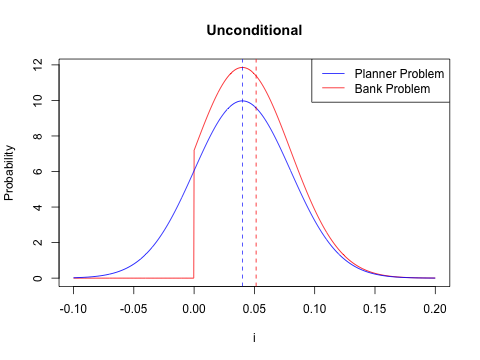
\includegraphics[scale=0.7]{ll_u}
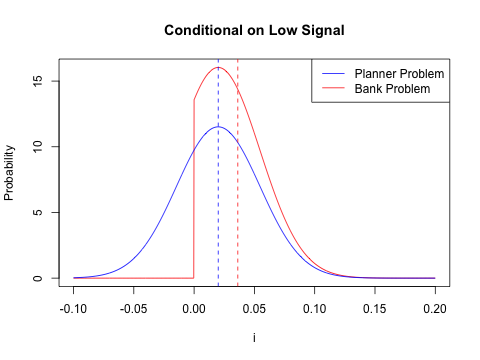
\includegraphics[scale=0.7]{ll_low}
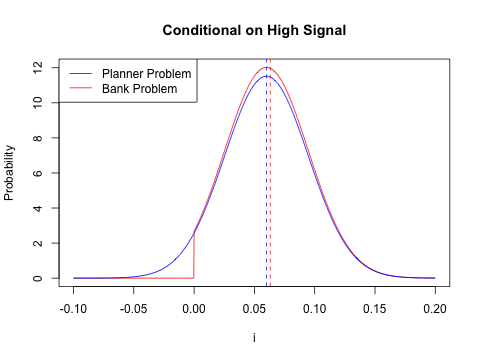
\includegraphics[scale=0.7]{ll_high}
\end{center}

\section{Estimation}

My plan is to estimate $\rho$ using simulated method of moment while using the rest of the parameters from Pandolfo ~\cite{pandolfo_2021}.  In particular, Pandolfo ~\cite{pandolfo_2021} estimates and/or calibrates $\mu = 0.04$, $\sigma = 0.04$, $\beta = 0.99$ (equivalently, $R = 1.01$), $\xi = 0.65$, and $\theta = 0.03$. Importantly, Pandolfo (2021) estimates these parameters using data from before the Dodd-Frank Act (DFA) and uses the pre-DFA level of capital requirement of $\phi = 0.04$.

\bigskip

To estimate $\rho$, I plan to target the cross-sectional correlation between lagged loan growth and realized loan returns. This data moment is the natural choice because if banks are more informed about loan return, they should ex ante investment more and grow their loan portfolio, so the correlation between the realized loan returns and change in quantity of loans should be higher.  The motivation to lag loan growth is to address concerns of the simultaneity bias; that is, the banks is mechanically able to make more loan if current loans are return more. This data moment is easily computed from Call Report data.  This data moment also corresponds well to a model analogue:

$$
Corr \Bigg(\frac{L' - L}{L}, i' \Bigg)
$$

As a robustness check, I plan to estimate this correlation while controlling for bank characteristics including size. In particular, I am concerned that there may be nonconstant returns-to-scale that would affect the loan return (e.g., monitoring costs, administrative costs).

\section{Results}

For results, I plan to follow Pandolfo ~\cite{pandolfo_2021} and evaluate optimal capital requirements by varying $\phi$ and using household consumption as the relevant welfare measure.  Recall that banks pay households dividends but households also pay for bank failures through lump-sum taxes.  First, I plan to find optimal capital requirements with $\phi = 0$ which should approximate correspond to the case studied by Pandolfo ~\cite{pandolfo_2021}.  Second, I plan to find optimal capital requirements with $\rho$ estimated to match the correlation in lagged loan growth and loan returns. If the optimal capital requirements are similar for different levels of $\rho$, then it would suggest that Pandolfo ~\cite{pandolfo_2021} and other studies that use a similar exogenous loan production technology are appropriate approximations of a more complex technology where banks are better informed.  However, if resulting optimal capital requirement differ greatly, it would cast doubt on these papers policy recommendations.

\pagebreak

\bibliography{refs}{}
\bibliographystyle{plain}

\end{document}
